\documentclass[11pt]{article}
\usepackage[margin=1in]{geometry}

\usepackage{graphicx}
\usepackage{caption}
\usepackage{subcaption}
\usepackage{placeins}
\usepackage{float}

\usepackage{amsmath}
\usepackage{hyperref}
\usepackage{parskip}
\usepackage{booktabs}

\captionsetup{labelfont=bf,font=small}
\graphicspath{{../figures/}}

\title{Bankruptcy Prediction Using Random Forest and XGBoost}
\author{Robert Hines}
\date{March 2026}

\begin{document}
\maketitle

\section{Introduction}

This report presents a binary classification study aimed at predicting company bankruptcy from historical financial and operational data. The business objective is to identify firms that will go bankrupt at some point within the observation window so that the organization can adjust investment and divestment decisions accordingly. The analysis does not target the exact timing of bankruptcy, only whether a company will eventually fail. The work relies on the Polish company bankruptcy dataset, which provides multiple annual snapshots over a five-year period. To mimic a real deployment scenario, the modeling pipeline trains on the fourth-year file and evaluates on the fifth-year file, treating the later year as genuinely ``future'' data rather than drawing a random split from a single file. Two tree-based estimators are implemented and evaluated: a Random Forest and an XGBoost classifier, both trained with cross-validation on the fourth-year data and assessed on the held-out fifth-year test set using ROC-AUC and confusion matrices. All preprocessing, model fitting, and evaluation were carried out in Python via \texttt{bankruptcy\_classifier.py} and are documented in the accompanying walkthrough notebook.

\section{Data and Preprocessing}

The data are supplied in ARFF format with 64 numeric attributes and a binary target indicating bankruptcy (class 1) or non-bankruptcy (class 0). The fourth-year file contains 9,792 samples; the fifth-year file contains 5,910 samples. Both years exhibit a strong class imbalance. In the fourth-year (training) data, approximately 94.7\% of companies are non-bankrupt and 5.3\% are bankrupt. In the fifth-year (test) data, approximately 93.1\% are non-bankrupt and 6.9\% are bankrupt. Missing values appear throughout the feature matrices and are encoded as missing in the ARFF source; after loading they are represented as NaN. Median imputation was applied per feature, with the imputer fit on the fourth-year training data only and then applied to both the training and fifth-year test sets, so that no information from the hold-out year influences the imputed values.

Instead of drawing a random train--test split from a single file, the pipeline uses a temporal split: all fourth-year observations serve as the training set and all fifth-year observations as the test set. Within the training data, stratified cross-validation preserves the bankrupt versus non-bankrupt ratio inside each fold. After imputation, the fourth-year training data were standardized to zero mean and unit variance using a StandardScaler, and the same transformation was applied to the fifth-year test set.

\section{Random Forest}

A Random Forest classifier was trained with the number of trees fixed at 300 and not tuned. Class weight was set to balanced to mitigate the effect of class imbalance on learning. Out-of-fold predictions were produced using stratified 5-fold cross-validation on the fourth-year training data. Under this baseline configuration, the model achieved an out-of-fold ROC-AUC of approximately 0.885 on the training folds and 0.949 on the fifth-year test set.

Hyperparameter tuning was performed over four parameters, each with five candidate values: \texttt{max\_depth}, \texttt{min\_samples\_split}, \texttt{min\_samples\_leaf}, and \texttt{max\_features}. A full grid of 625 configurations was evaluated with stratified 5-fold cross-validation and ROC-AUC as the scoring metric. The selected configuration was \texttt{max\_depth} None, \texttt{min\_samples\_split} 2, \texttt{min\_samples\_leaf} 4, and \texttt{max\_features} 0.7, yielding a best tuning CV mean ROC-AUC of approximately 0.918, an out-of-fold ROC-AUC of approximately 0.917 on the training folds, and a test-set ROC-AUC of approximately 0.966. Table~\ref{tab:rf_tuning} summarizes the top tuning results.

\begin{table}[!htbp]
\centering
\caption{Top Random Forest hyperparameter configurations by tuning CV mean ROC-AUC.}
\label{tab:rf_tuning}
\begin{tabular}{lllllc}
\toprule
Rank & max\_depth & min\_samples\_split & min\_samples\_leaf & max\_features & CV ROC-AUC \\
\midrule
1 & None & 2 & 4 & 0.7 & 0.9179 \\
2 & None & 5 & 4 & 0.7 & 0.9179 \\
3 & 40 & 2 & 4 & 0.7 & 0.9179 \\
4 & 40 & 5 & 4 & 0.7 & 0.9179 \\
5 & 40 & 2 & 2 & 0.7 & 0.9179 \\
\bottomrule
\end{tabular}
\end{table}
\FloatBarrier

\section{XGBoost}

An XGBoost classifier was trained with early stopping so that the effective number of boosting rounds is determined by validation performance rather than by tuning the round count directly. A maximum of 1000 rounds was set and early stopping halted training when validation AUC did not improve for 50 rounds. A dedicated validation split from the fourth-year training data was used for early stopping during the baseline run, hyperparameter search, and final tuned model fit. Out-of-fold predictions for the tuned configuration were obtained with stratified 5-fold cross-validation and early stopping inside each fold.

Hyperparameter tuning sampled 40 configurations from a six-dimensional grid (five values per parameter) and evaluated each with stratified 3-fold cross-validation and early stopping in every fold. The best configuration found was \texttt{max\_depth} 8, \texttt{learning\_rate} 0.07, \texttt{min\_child\_weight} 1, \texttt{subsample} 0.9, \texttt{colsample\_bytree} 0.9, and \texttt{reg\_lambda} 0.0, with a tuning CV mean ROC-AUC of approximately 0.939. After refitting with early stopping, the tuned model reached a validation ROC-AUC of approximately 0.943, an out-of-fold training ROC-AUC of approximately 0.937, and a fifth-year test ROC-AUC of approximately 0.971. The baseline XGBoost reached a validation ROC-AUC of approximately 0.926 and a test ROC-AUC of approximately 0.968. Table~\ref{tab:xgb_tuning} summarizes the top five configurations from the sampled search.

\begin{table}[!htbp]
\centering
\caption{Top five XGBoost hyperparameter configurations from the sampled grid search.}
\label{tab:xgb_tuning}
\begin{tabular}{lllllllc}
\toprule
Rank & max\_depth & lr & min\_child & subsample & colsample & reg\_lambda & CV ROC-AUC \\
\midrule
1 & 8 & 0.07 & 1 & 0.9 & 0.9 & 0.0 & 0.9392 \\
2 & 6 & 0.03 & 1 & 0.8 & 0.6 & 0.5 & 0.9371 \\
3 & 8 & 0.01 & 5 & 0.9 & 1.0 & 0.0 & 0.9360 \\
4 & 6 & 0.03 & 3 & 0.9 & 0.6 & 1.5 & 0.9358 \\
5 & 5 & 0.07 & 1 & 0.9 & 0.8 & 0.0 & 0.9358 \\
\bottomrule
\end{tabular}
\end{table}
\FloatBarrier

\section{Results}

Figure~\ref{fig:roc} shows the ROC curves for the baseline Random Forest, the tuned Random Forest, and the tuned XGBoost on the held-out fifth-year test set. The baseline Random Forest reaches a test ROC-AUC of approximately 0.949, the tuned Random Forest approximately 0.966, and the tuned XGBoost approximately 0.971. Confusion matrices for the tuned models were computed at a probability threshold of 0.5 (Figures~\ref{fig:cm_rf} and~\ref{fig:cm_xgb}).

\begin{figure}[!htbp]
\centering
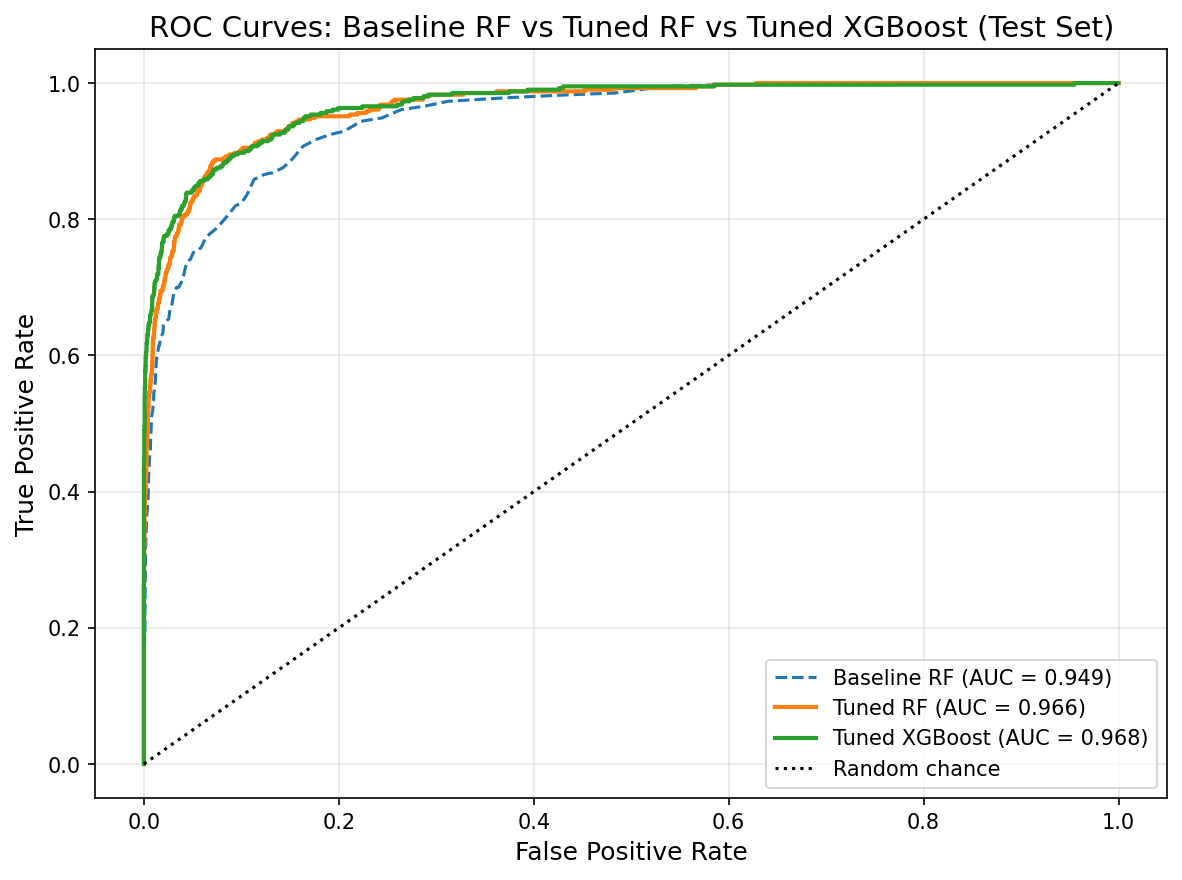
\includegraphics[width=0.85\textwidth]{roc_curves_baseline_rf_tuned_rf_xgb.png}
\caption{ROC curves on the fifth-year test set.}
\label{fig:roc}
\end{figure}

\begin{figure}[!htbp]
\centering
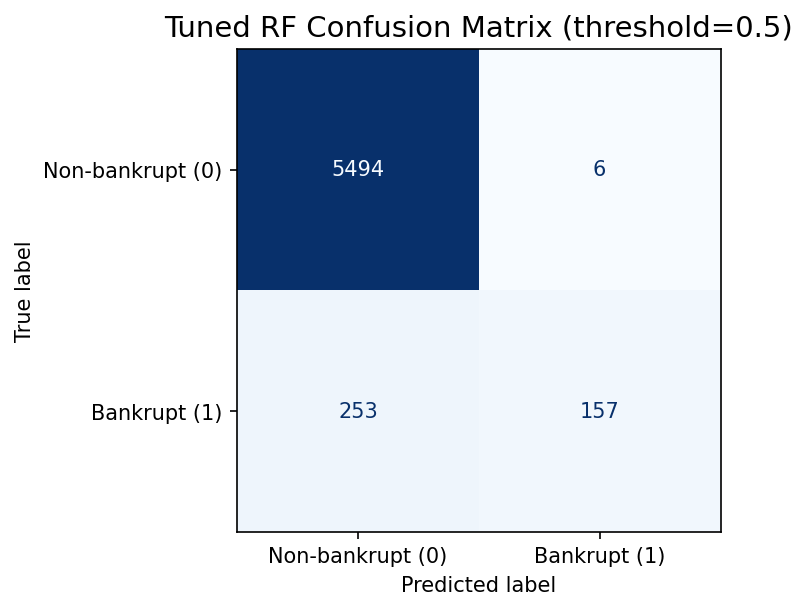
\includegraphics[width=0.6\textwidth]{confusion_matrix_rf.png}
\caption{Confusion matrix for the tuned Random Forest (threshold 0.5).}
\label{fig:cm_rf}
\end{figure}

\begin{figure}[!htbp]
\centering
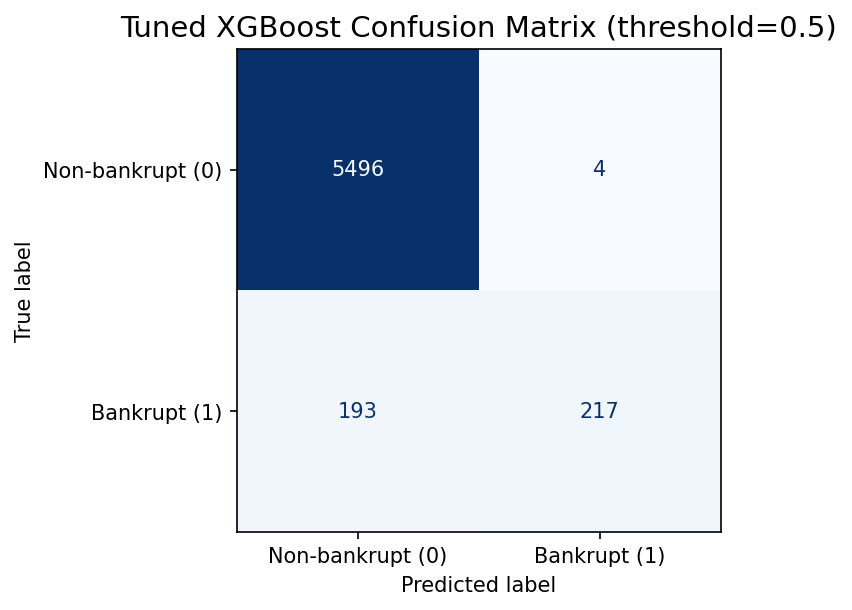
\includegraphics[width=0.6\textwidth]{confusion_matrix_xgb.png}
\caption{Confusion matrix for the tuned XGBoost (threshold 0.5).}
\label{fig:cm_xgb}
\end{figure}

\FloatBarrier

\section{Discussion}

The Polish company bankruptcy dataset has been studied extensively; reported AUC values often fall in the high 0.80s to mid 0.90s depending on horizon, preprocessing, and evaluation protocol. The present results---tuned Random Forest test AUC approximately 0.966 and tuned XGBoost approximately 0.971 under a temporal 4$\rightarrow$5 split---are strong relative to many published benchmarks, though direct comparison requires matching the same split and preprocessing choices. Test AUC exceeding training cross-validation AUC may reflect a slightly higher bankrupt rate in the fifth-year cohort and distributional shift between years. Both models provide usable risk rankings; XGBoost offers a modest AUC advantage while Random Forest may be preferable when interpretability of individual trees matters.

\section{Conclusion}

This project implements a reproducible bankruptcy prediction pipeline with median imputation, temporal train/test separation, and standardized features fit on the training year only. Random Forest and XGBoost models were tuned under fixed tree-count and early-stopping constraints and evaluated with ROC-AUC and confusion matrices.

The pipeline is packaged for reuse via \texttt{bankruptcy\_classifier.py}. The accompanying notebook provides a phase-by-phase walkthrough of the same code path.

\end{document}
